\documentclass[12pt]{article}

\usepackage[utf8]{inputenc}
\usepackage{geometry}
\geometry{a4paper,scale=0.75}
\linespread{1.5}
\usepackage{graphicx} 
\usepackage{float} 
\usepackage{subfig} 
\usepackage{enumerate}
\usepackage{enumitem}
\usepackage{amsmath}
\usepackage{array}
\usepackage{booktabs}
\usepackage{multirow}
\usepackage{amsfonts}
\usepackage[english]{babel}
\usepackage{amsthm}
\usepackage{dcolumn}
\usepackage{multicol}
\usepackage{stfloats}
\usepackage{lscape}
\usepackage[figuresright]{rotating}
\RequirePackage{pdflscape}
\usepackage[toc,page]{appendix}
\usepackage{geometry}
\usepackage{longtable}
\usepackage{comment}
\usepackage{xcolor}

% -------- enumerated sub-labels (a), (b), … --
\usepackage{enumitem}
\setlist[enumerate,1]{label=(\alph*),ref=\alph*}
% ---------------------------------------------

\usepackage{hyperref}
\hypersetup{hidelinks,
	colorlinks=true,
	allcolors=black,
	pdfstartview=Fit,
	breaklinks=true}
\usepackage{csquotes}
\usepackage{natbib}
\bibliographystyle{apalike}
\newtheorem{definition}{Definition}
\newtheorem{theorem}{Theorem}
\newtheorem{proposition}[theorem]{Proposition}
\newtheorem{lemma}[theorem]{Lemma}
\newtheorem{corollary}[theorem]{Corollary}
\newtheorem*{remark}{Remark}
\newtheorem{example}{Example}
\newtheorem{exercise}{Exercise}
\newtheorem{assumption}{Assumption}[section] % number within sections


\begin{document}

\begin{center}
    ECON 3123: Macroeconomic Theory I\\
    {\large \textbf{Tutorial Note 6: Labour Market and Phillips Curve}}\\
    Teaching Assistant: Harlly Zhou
\end{center}

\subsection*{A Simple Model of the Labour Market}
\paragraph{Price Determination} Consider a production function
\[Y = AN.\]
The \textbf{marginal product of labour} (MPL) is $\frac{\partial Y}{\partial N} = A$. Suppose that the cost of hiring an extra worker is $W$. Then the marginal cost of production is $\frac{W}{A}$. Let $m$ be the markup (due to monopolistic power). Then the price level will be
\[ P = (1+m)\frac{W}{A}.\]

\paragraph{Wage Determination} Assume that the nominal wage is
\[W = A P^e F(u,z),\]
where $A$ is the MPL, $P^e$ is the expected price level, and $F$ is a function decreasing in unemployment rate $u$, and increasing in $z$, a variable capturing all other factors.

\paragraph{Natural Rate of Unemployment} From the price determination equation, we have
\[\frac{W}{P} = \frac{A}{1+m}.\]
From the wage determination equation, we have
\[\frac{W}{P} = AF(u,z).\]
In a $\left(u, \frac{W}{P}\right)$ diagram, the pricing curve is a horizontal line, and the wage curve is a downward-sloping curve, as is shown in Figure \ref{fig:wu_01}.

\begin{figure}[htp]
    \centering
    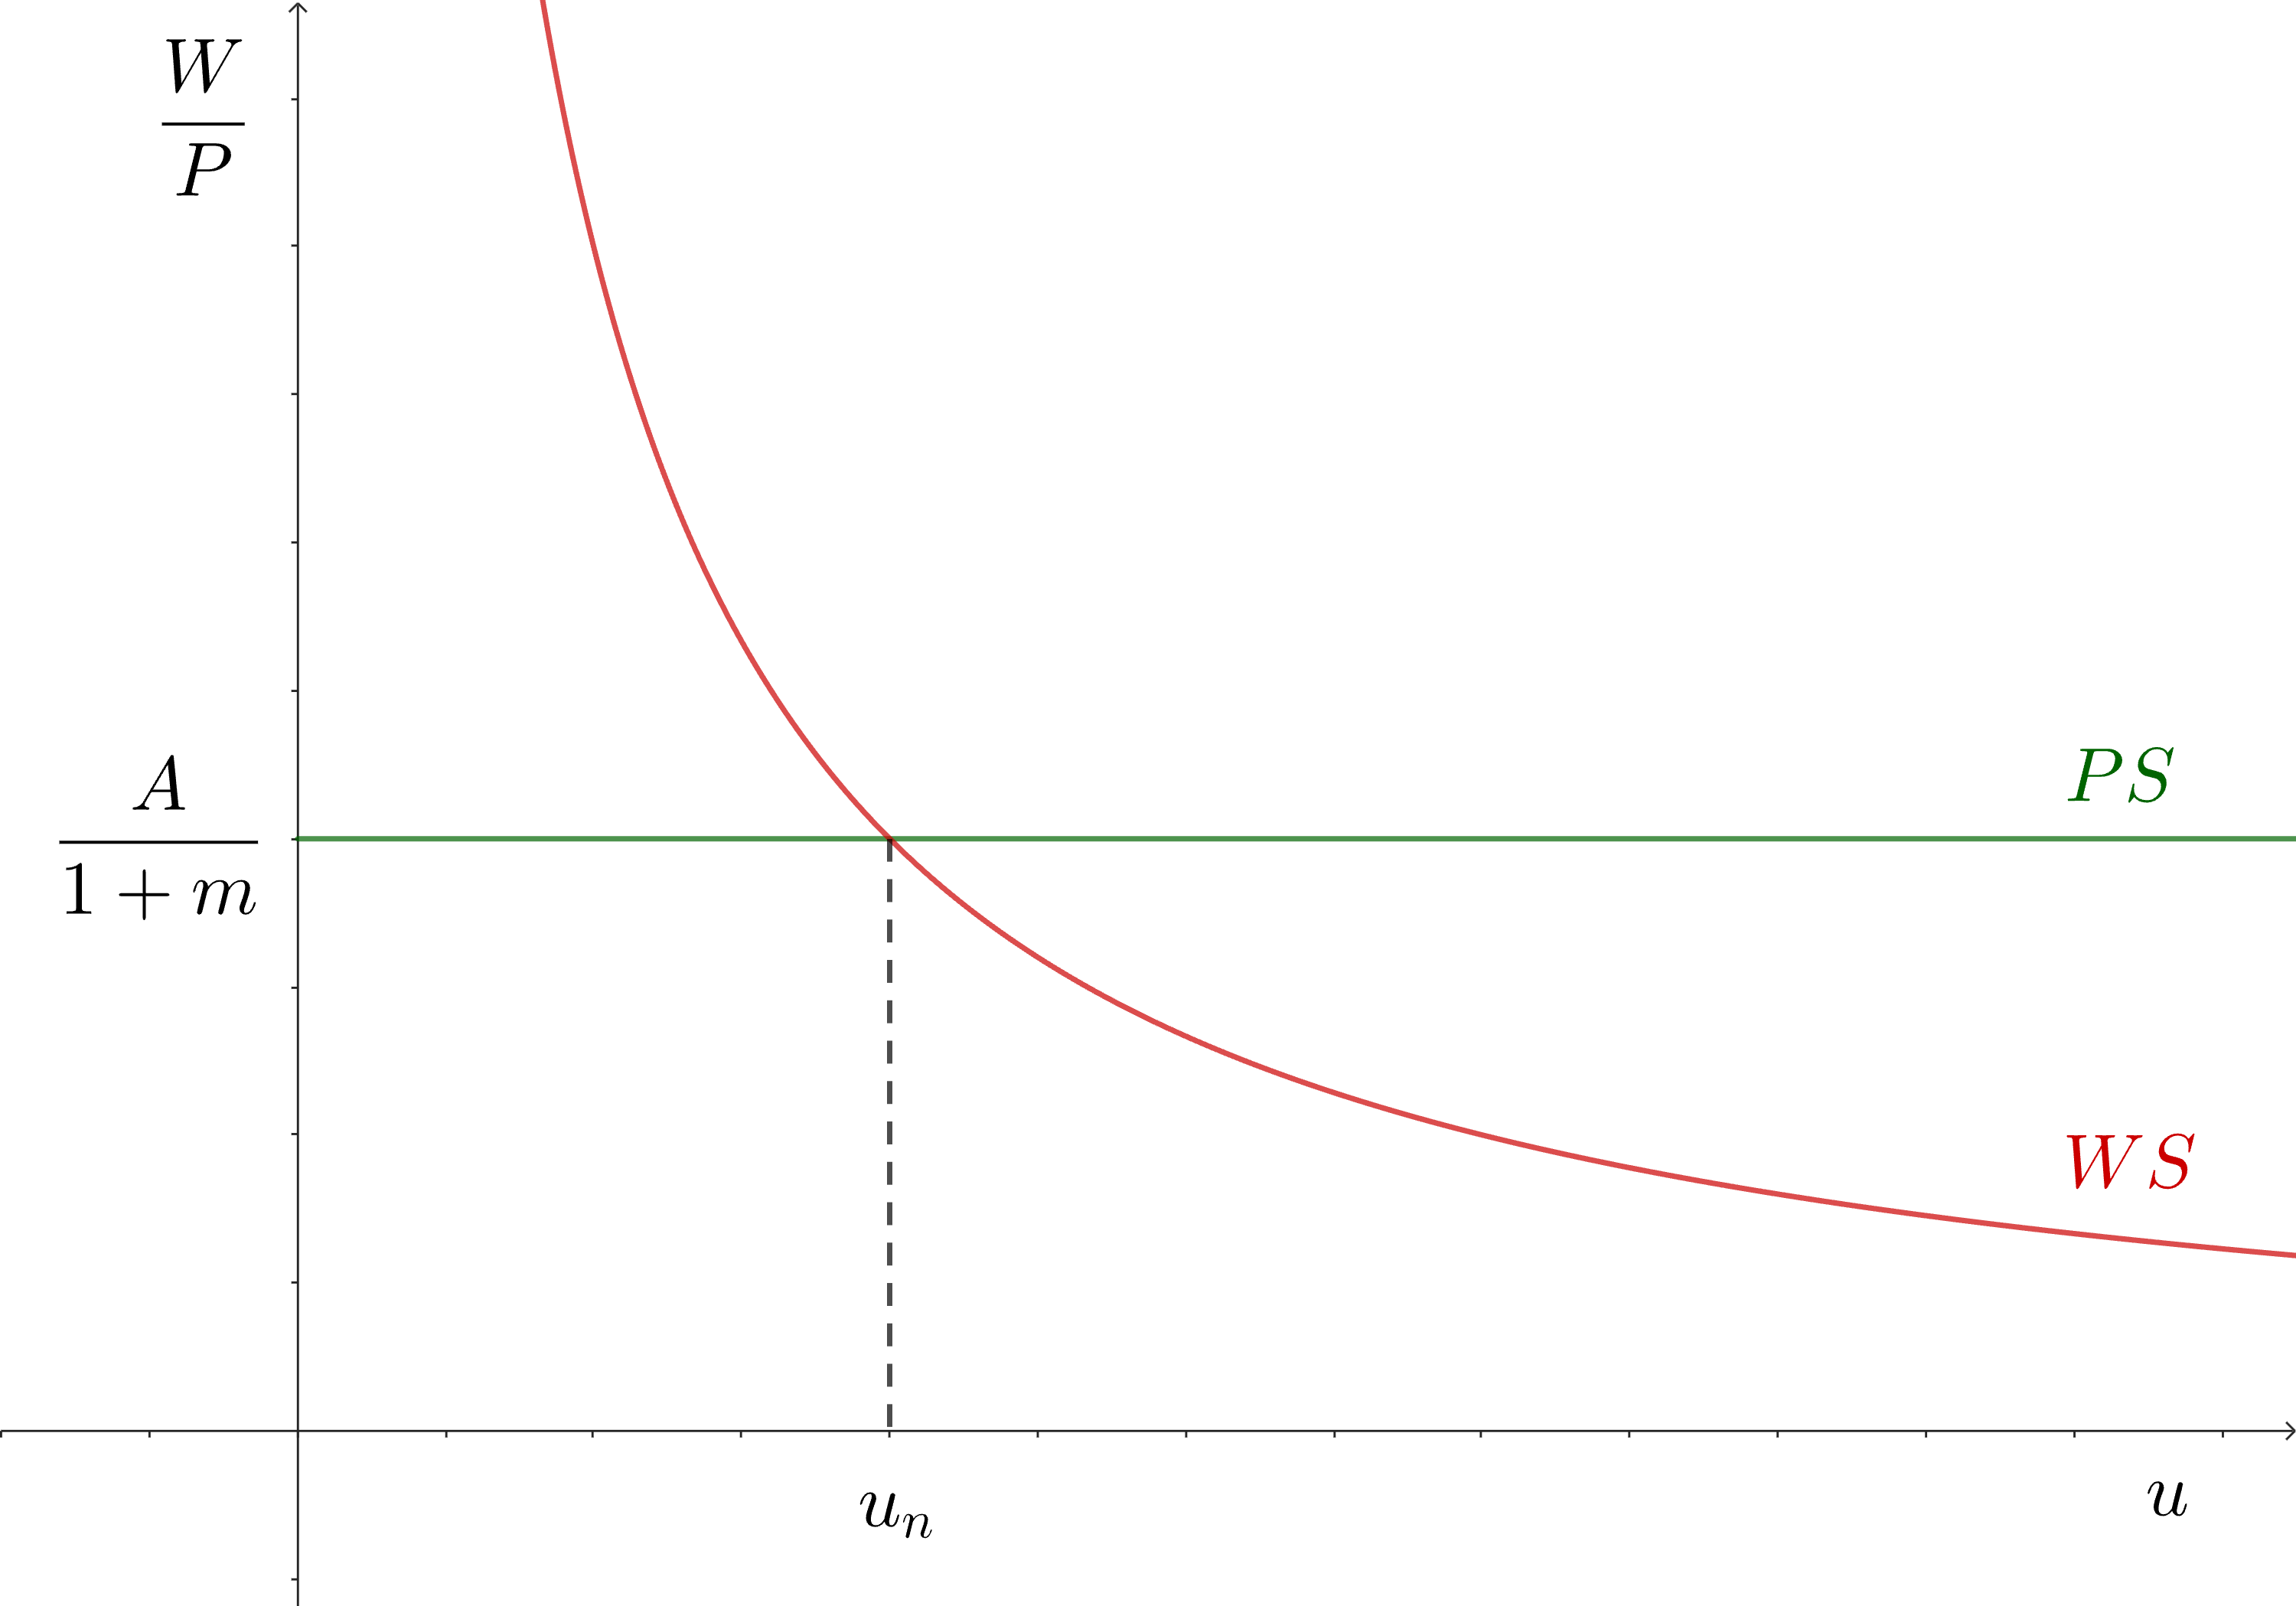
\includegraphics[width=0.6\textwidth]{wu_01.png}
    \caption{Natural Rate of Unemployment}
    \label{fig:wu_01}
\end{figure}

\end{document}